\documentclass{article}
\usepackage{graphicx}
\usepackage{float}
\parskip=12pt

\begin{document}

\title{Laboratory 2: DC and AC Circuits}
\date{October 29, 2014}
\author{Calvin Chan\\304144970\\Physics 4BL Lab 8\\Partners: Caleb Choi, Stanley
Chan}

\maketitle

\section{Introduction}
This lab analyzes the properties of DC and AC circuits by examining the basic
properties of resistors, diodes, capacitors, and inductors and constructing the
two circuits with said components. The lab will examine the current-voltage
characteristics of various load devices – the lab will look at resistors
(individually, in series, and in parallel) and diodes and examine whether all
load devices fall under Ohm's law. The AC portion of the lab will look at two
reactive components capacitors and inductors and the transient states of
circuits with those load devices.

\section{Experimental Results}

\subsection{DC Circuits: Ohm's Law}

\begin{enumerate}
    \item Build a circuit with two resistors in series, one with a known
    resistance value and another with an unknown value.
    \item Connect a voltage meter to measure the voltage drops through both
    resistors.
    \item Connect the circuit to the ADC. Apply a max voltage of 5V and retrieve
    a sample size of 1,000 points using a sampling rate of 5000 samples/sec.
\end{enumerate}

For the first part of the lab, we want to analyze the current-voltage
characteristic of a single resistor as our load device. We can use an IV curve
to track how much current flows through the resistor at varying voltages, and
thus, verifying Ohm's law \textbf{(eq. \ref{ohms_law})} by generating an IV
curve for the simple resistor \textbf{(fig. \ref{ivcurve_simpleresistor})}. 

\begin{equation}
    \label{ohms_law}
    I(V) = \frac{V}{R}
\end{equation}

\begin{figure}[H]
    \centering
    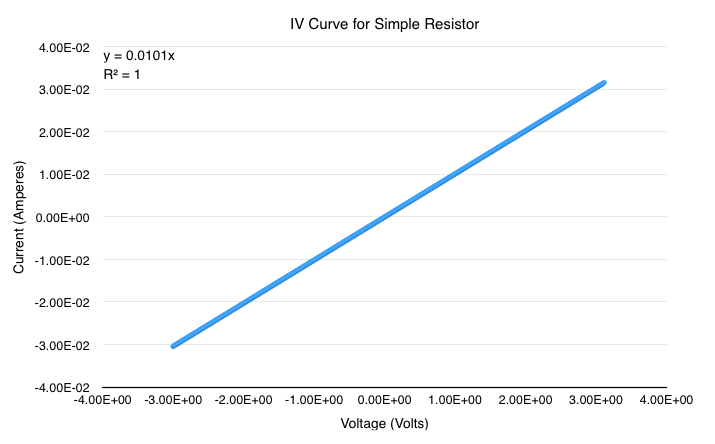
\includegraphics[width=\textwidth]{charts/ivcurve_simpleresistor}
    \caption{IV Curve for a resistor of unknown resistance}
    \label{ivcurve_simpleresistor}
\end{figure}

We used a known resistor of 98.8 $\Omega$ and connected it in series with
another resistor of unknown resistance. Using Ohm's law \textbf{(eq.
\ref{ohms_law})}, the current through the entire circuit was calculated at each
varying voltage.

\subsection{DC Circuits: Deviation from Ohm's Law}

\begin{enumerate}
    \item Build a circuit with a resistor and a diode connected in series.
    \item Connect a voltage meter to measure the voltage drops through both, the
    resistor and the diode.
    \item Connect the circuit to the ADC. Apply a max voltage of 5V and retrieve
    a sample size of 1,000 points using a sampling rate of 5000 samples/sec.
\end{enumerate}

Next, we want to analyze the current-voltage characteristic of a diode as our
load device. We can use an IV curve to track how much current flows through the
diode at varying voltages. Unlike resistors, diodes only allow current to flow
in a single direction when a tiny voltage is applied. 

For this part of the lab, we used a known resistor of 98.8 $\Omega$ and
connected it in series with a diode. Using Ohm's law \textbf{(eq.
\ref{ohms_law})}, the current through the entire circuit was calculated at each
varying voltage.

\begin{figure}[H]
    \centering
    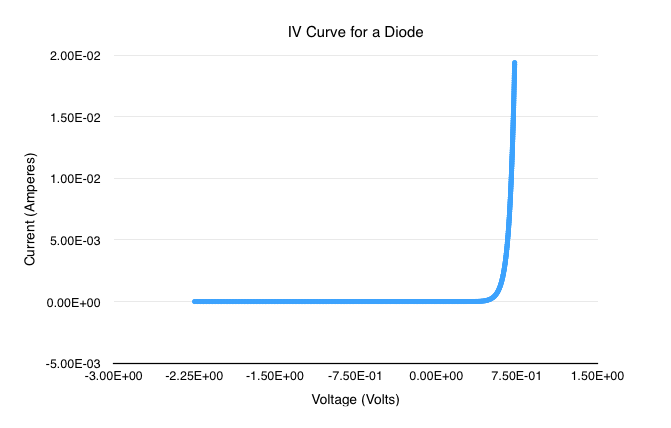
\includegraphics[width=\textwidth]{charts/ivcurve_diode}
    \caption{IV Curve for a diode}
    \label{ivcurve_diode}
\end{figure}

\subsection{AC Circuits: RC Transient State}

\begin{enumerate}
    \item Select a resistor and capacitor and connect them in series.
    \item Ensure that the selecte resistor and capacitor yield a time constant
    of roughly $10^{-3}$ seconds.
    \item Use a voltage generator to generate a voltage with a square waveform
    with a frequency of roughly $10 Hz$ and a voltage amplitude of about $2 V$.
    \item Use the voltmeter to measure the voltage drop across the resistor and
    the capacitor, collecting a total of 1000 points with a sampling rate of
    5000 points/sec.
\end{enumerate}

For this part of the lab, we want to analyze the transient states of a circuit
that involves uses a capacitor as the load device. We can monitor the input
voltage and compare it to the voltage drop across the capacitor over time, as
shown in \textbf{fig.(\ref{rccurve_transient})}. Evidently, the voltage across
the capacitor is initially very small, and increases rapidly as it charges. It
eventually reaches a steady state, at which it is near full charge.

\begin{figure}[H]
    \centering
    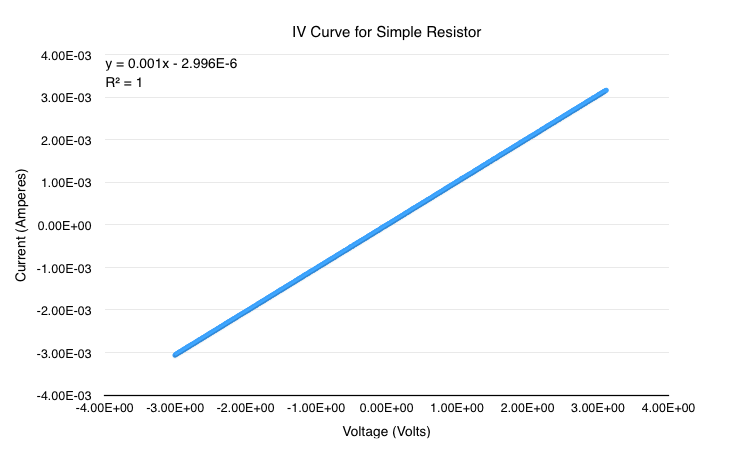
\includegraphics[width=\textwidth]{charts/rccurve_transient}
    \caption{Voltage across the capacitor during the transient state period}
    \label{rccurve_transient}
\end{figure}

We used a known resistor of 1000 $\Omega$ and connected it in series with
a capacitor of 1 $\mu F$.

\subsection{AC Circuits: RL Transient State}

\begin{enumerate}
    \item Build a circuit with two resistors in parallel, connected to an
    inductor in series.
    \item Select a resistor and capacitor and connect them in series.
    \item Ensure that the selecte resistor and capacitor yield a time constant
    of roughly $10^{-3}$ seconds.
    \item Use a voltage generator to generate a voltage with a square waveform
    with a frequency of roughly $1 Hz$ and a voltage amplitude of about $2 V$.
    \item Use the voltmeter to measure the voltage drop across the resistor and
    the capacitor, collecting a total of 2000 points with a sampling rate of
    2000 points/sec.
\end{enumerate}

\begin{figure}[H]
    \centering
    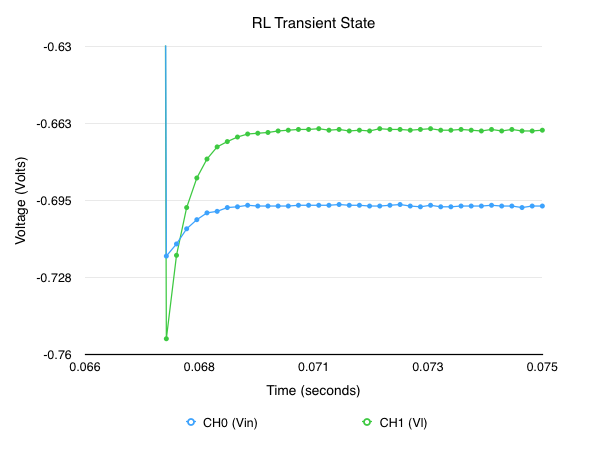
\includegraphics[width=\textwidth]{charts/rlcurve_transient}
    \caption{Voltage across the inductor during the transient state period}
    \label{rlcurve_transient}
\end{figure}

Similar to the RC portion of the lab, we want to analyze the transient states of
a circuit that involves uses an inductor as the load device. We can monitor the
input voltage and compare it to the voltage drop across the inductor over time,
as shown in \textbf{fig.(\ref{rlcurve_transient})}. The transient state of the
circuit exists where there is a significant voltage jump from low to high. This
is where the current changes. There was a shortage of components during the lab
session, so the data was provided by the TA.

\subsection{AC Circuits: RLC Resonance}

\begin{enumerate}
    \item Build a circuit with a capacitor, an inductor, and a resistor, all
    connected in series.
    \item Use a resistor of roughly $1000\Omega$, and the biggest value
    capacitor and resistor
    \item Connect the circuit to the myDAQ and configure the Bode Analyzer to
    use a start frequency of roughly $10Hz$, a stop frequency of roughly $20Hz$,
    10 steps per decade, and a peak amplitude of $2V$.
\end{enumerate}

\begin{figure}[H]
    \centering
    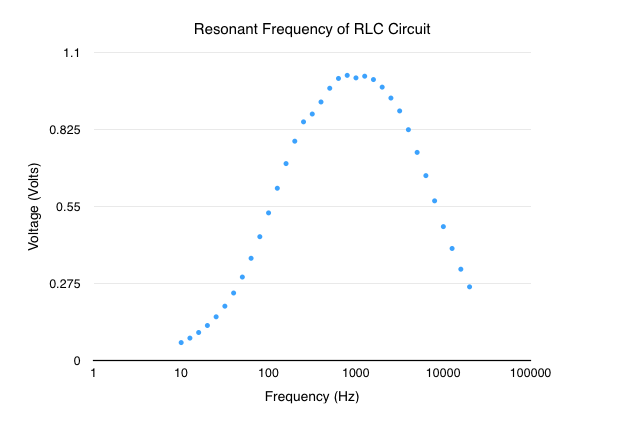
\includegraphics[width=\textwidth]{charts/rlccurve_resonant}
    \caption{The resonant frequency of a RLC circuit}
    \label{rlccurve_resonant}
\end{figure}

For the RLC circuit, we used an inductor of $30mH$, a resistor of $1000\Omega$
and a capacitor of $1\mu F$. We want to analyze the circuit to determine at what
frequency it reaches it's peak voltage output. As shown in the figure
\ref{rlccurve_resonant}, the voltage peaks as the frequency approaches the
resonant frequency, but drops as the frequency overshoots the resonance point.

\section{Analysis}

\subsection{DC Circuits: Ohm's Law}

The range of the IV Curve \textbf{(fig. \ref{ivcurve_simpleresistor})} contains
the current values (in Amperes) per domain value, the voltage (in Volts)
measured across the unknown resistor. As such, the curve displays a linear
relationship between the current and voltage, successfully verifying Ohm's law
and proving that voltage and current are directly proportional.

Using the linear regression we performed in \textbf{fig.
\ref{ivcurve_simpleresistor}}, we find that the slope of the line is $m =
0.001014$ with an error of $7.53 x 10^{-7}$. Inverting the slope gives us the
experimental resistance of the unknown resistor.

\begin{equation}
    \label{ohms_law_slope}
    R = \frac{1}{m} = \frac{1}{0.001014} = 985.7
\end{equation}

We also used a multimeter to measure the theoretical value of the "unknown"
resistor, which yielded $985\pm0.5\Omega$. To compare our experimental values
with the theoretical values, the percent error formula can be used:

\begin{equation}
    \label{percent_error}
    error = \frac{theoretical-experimental}{experimental}
\end{equation}
\begin{equation}
    \label{error_ohms_law_2}
    error = \frac{|985-985.7|}{985.7}
    error = 0.07\%
\end{equation}
\begin{equation}
    \label{error_ohms_law_3}
    error = 0.07\%
\end{equation}


\subsection{DC Circuits: Deviation from Ohm's Law}

The range of the IV Curve for a diode \textbf{(fig. \ref{ivcurve_diode})}
contains the current values (in Amperes) per domain value, the voltage (in
Volts) measured across the diode. From the graph, we can see that diodes deviate
from Ohm's law \textbf{(eq. \ref{ohms_law})} because voltage and current are not
directly proportional through the graph. In fact, the diodes are a non-ohmic
load device that exhibit exponential dependence; the current that
flows through a diode can be found using the following equation:

\begin{equation}
    \label{iv_diode}
    I(V) = I_{0}(e^{e^{\frac{|e|V}{nk_{B}T}}}-1)
\end{equation}

To analyze this further, we must first linearize the data to perform linear
regression. We determine the value of the diode constant to be the value of the
current when the applied voltage is the lowest: $I_{0} = 7.14 x 10^{-6}$. Next
we can linearize \textbf{eq. \ref{iv_diode}} by taking the natural log of both
sides, simplified under the assumption that $I+I_{0}=I$ because the diode
constant is so much smaller than all of our other measured current values:

\begin{equation}
    \label{iv_diode_linearized}
    ln(I) = ln(I_{0})+\frac{|e|}{nk_{B}T}V
\end{equation}

\begin{figure}[H]
    \centering
    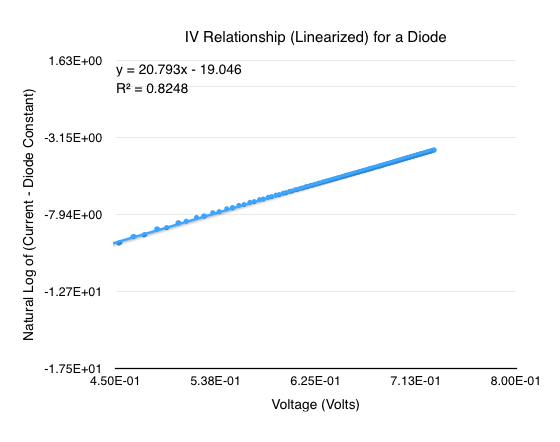
\includegraphics[width=\textwidth]{charts/ivcurve_diode_linear}
    \caption{Linearized IV Curve for a diode}
    \label{ivcurve_diode_linearized}
\end{figure}

From performing the linear regression as shown in \textbf{fig.
\ref{ivcurve_diode_linearized}}, we can determine the value of the ratio
$\frac{e}{nk_{B}T}$ to be the value of the slope ($m=20.793$) with an error of
$0.043213$, shown in \textbf{eq. \ref{boltzmann_analysis_1}}. Using $n=2$ and
$T=293K$, we can further simplify the ratio to determine $\frac{e}{k_{B}}$, the
charge of an electron and the Boltzmann constant, which are two fundamental
constants of nature \textbf{(eq. \ref{boltzmann_analysis_2})}.

\begin{equation}
    \label{boltzmann_analysis_1}
    \frac{e}{nk_{B}T} = {20.793}
\end{equation}
\begin{equation}
    \label{boltzmann_analysis_2}
    \frac{e}{k_{B}} = 2\cdot293\cdot20.793 = 12184.698
\end{equation}

Since we know the value of the charge of an electron and the Boltzmann constant,
we can calculate the theoretical value of the ratio:

\begin{equation}
    \label{boltzmann_analysis_3}
    \frac{e}{k_{B}} = \frac{1.602\cdot10^{-19}C}{1.381\cdot10^{-23}J/K} =
    11604.519
\end{equation}

And next, we can calculate the error in our measurements using the percent error
formula \textbf{(eq. \ref{percent_error})}:

\begin{equation}
    \label{boltzmann_err_analysis_1}
    error = \frac{|11604.519-12184.698|}{12184.698} = 4.76\%
\end{equation}

We had a relatively small margin of error, which could be justified by the
number of useless data points provided by values at low voltages. These data
points were created because at small and negative values of voltage, the
exponential relationship is not strong, thus disrupting the regression.

\subsection{AC Circuits: Linear Regression of RC Circuit}

The voltage across a capacitor can be derived into a function with respect to
time:

\begin{equation}
    \label{rc_eq_1}
    V_{C}(t)=V_{b}(1-e^{\frac{-t}{RC}})
\end{equation}

Furthermore, in a RC circuit, the time scale of transition between the transient
and steady state can be defined by the previous equation \textbf{(eq.
\ref{rc_eq_1})}:

\begin{equation}
    \label{rc_timescale}
    \tau=RC
\end{equation}

We can perform linear regression on the data we collected to identify the
measured characteristic time scale of the transient RC circuit. Linearizing
equation \ref{rc_eq_1} yields the following:

\begin{equation}
    \label{rc_eq_1_linear}
    ln(V_{b}-V)=ln(V_{b})-\frac{1}{RC}t
\end{equation}

From the previous equation \textbf{eq. \ref{rc_eq_1_linear}}, we see that the
value of the slope ($m=-934.35$) from our linear regression is $1/RC$. Thus, the
measured value of our time constant is:

\begin{equation}
    \label{rc_timescale_measured}
    \tau=RC=-\frac{1}{-934.35}=0.00107
\end{equation}

Given that we know the actual values of both $R=985\pm0.5\Omega$ and $C=1\mu F$, we
can calculate the theoretical value of the time constant \textbf{eq.
\ref{rc_timescale_theoretical}} and, sequentially, the error in our measurements
using the percent error equation \textbf{(eq. \ref{percent_error})}:

\begin{equation}
    \label{rc_timescale_theoretical}
    \tau_{theoretical}=985\cdot(1\cdot10^{-6})=0.000985
\end{equation}

\begin{equation}
    \label{rc_err_analysis}
    error=\frac{|0.000985-0.00107|}{0.00107}=7.94\%
\end{equation}

\subsection{AC Circuits: RLC Resonance}

From looking at the graph of the RLC circuit \textbf{(fig.
\ref{rlccurve_resonant})}, we can see that the resonant frequency is at about
$1000 Hz$, which gives us our measured value for $f_{res}$.

Given that we know the actual values of our inductor ($30mH$) and capacitor
($1\mu F$), we can
calculate the theoretical resonant frequency of the circuit using the following
equation:

\begin{equation}
    \label{resonant_frequency_1}
    f_{res}=\frac{1}{2\pi\sqrt{LC}}
\end{equation}
\begin{equation}
    \label{resonant_frequency_2}
    f_{res}=\frac{1}{2\pi\sqrt{(30\cdot10^{-3})(1\cdot10^{-6})}}
\end{equation}
\begin{equation}
    \label{resonant_frequency_3}
    f_{res}=918.88Hz
\end{equation}

Once again using the percent error equation \textbf{(eq. \ref{percent_error})}, we
can calculate the error in our measurements:

\begin{equation}
    \label{resonance_err_analysis}
    error=\frac{|1000-918.88|}{1000}=8.11\% \end{equation}

\subsection{AC Circuits: RLC Q-factor}

To find the Q-factor of the RLC circuit, we must first find the width of the
resonance peak and the power loss in the circuit. To do this, we find $V_{max}$
at $f_{res}$, then calculate $V_{max}/\sqrt{2}$ and find $f_{1}$ and $f_{2}$ where it intersects the
resonance curve \textbf{(fig. \ref{rlccurve_resonant})}. Finally, the Q-factor
can be determined by the following equation:

\begin{equation}
    \label{q_factor}
    Q = \frac{f_{res}}{f_{2}-f_{1}}
\end{equation}

\begin{figure}[H]
    \centering
    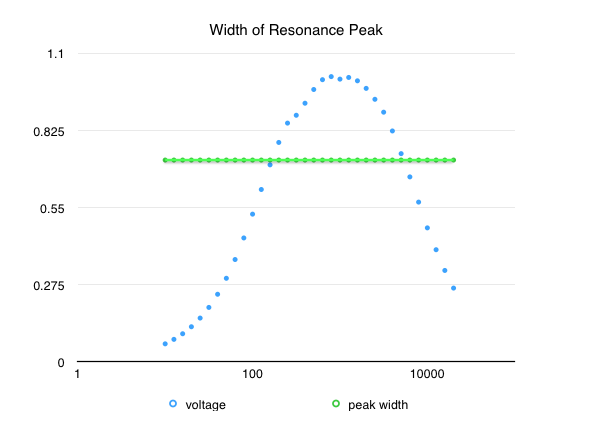
\includegraphics[width=\textwidth]{charts/rlccurve_resonant_width}
    \caption{Width of the resonance peak for the RLC circuit}
    \label{rlccurve_resonant_width}
\end{figure}

Using $V_{max}=1.017V$, we can determine where this intersects the resonance
curve \textbf{(fig. \ref{rlccurve_resonant})}. $f_{1}=158.489Hz$ and
$f_{1}=5011.872Hz$. Plugging these into \textbf{eq. \ref{q_factor}}:

\begin{equation}
    \label{q_factor_1}
    Q = \frac{1000}{5011.872-158.489}=\frac{1000}{4853.383}=0.206
\end{equation}

\section{Conclusion}
Upon completion of the lab, we were able to achieve most of our main objectives.
The DC circuit with a single resistor showed the Ohm's law was indeed correct
for simple load devies, generating a linear, direct correlation between current
and voltage. However we also showed that certain load devices (such as a diode,
in our case) did that fall under Ohm's law, but rather, exhibited other
non-linear properties. The diode in particular had an exponential relationship
between current and voltage.

The AC portion of the lab examined the transient states of various circuits. In
observing the RC circuit, we noticed the capacitor rapidly charging in the
beginning of each period, eventually reaching a steady state. By linearizing the
relationship between the current and the voltage, we were able to determine the
time constant value for the transient state. Finally, the RLC circuit showed the
correlation between frequency and voltage, and how the resonant frequency at
which the voltage is greatest in the circuit determines the Q-factor of the
circuit itself.
\end{document}
